\documentclass[xcolor=dvipsnames]{beamer}

% font setup
\usepackage{libertine}
\renewcommand*\familydefault{\sfdefault}    % Linux Libertine = default sans serif
\usepackage{inconsolata}                    % Inconsolata = monospaced
\usepackage[utf8]{inputenc}
\usepackage[T1]{fontenc}
\usepackage{tikz}
\usetikzlibrary{positioning}
\usepackage[style=german]{csquotes}
\newcommand\qq{\enquote}
\newcommand\dr{\mathrm}
\usepackage[normalem]{ulem}

\usepackage{algorithm}
\usepackage{algpseudocode}
\makeatletter
\renewcommand{\ALG@name}{Algoritm}
\makeatother
\algrenewcommand\algorithmicprocedure{\textbf{procedură}}
\algrenewcommand\algorithmicend{\textbf{final}}

% Graphics and other packages
\usepackage[romanian]{babel}
\usepackage{graphicx}
\addto\captionsromanian{\renewcommand{\figurename}{Ilustrație}}
\usepackage{caption}
\usepackage{subcaption}
\usepackage[style=german]{csquotes}

% Custom macros
\newcommand{\bloc}[3]{\begin{bl}<#1->{{\large\color{Gray}{\hrulefill}}\\ \color{bleumarin}{\large \emph{#2}}}\\ \vspace*{-2mm}{\color{Gray}{\hrulefill}}\\ #3 \end{bl}} 
\newcommand{\fr}[1]{\frame{#1}}
\newcommand{\ft}[1]{\frametitle{\color{bleumarin}{\hfill #1 \hfill}}}
\newcommand{\lin}[3]{\uncover<#1->{\alert<#1>{#2}}{\vspace*{#3 ex}}}
\newcommand{\ite}[2]{\uncover<#1->{\alert<#1>{\item #2}}}
\newcommand{\vs}[1]{\vspace*{#1 ex}}
\definecolor{bleumarin}{RGB}{30,30,150} 
\definecolor{firebrick}{RGB}{178,34,34}

% Theme setup
\useoutertheme{shadow} 
\usetheme{CambridgeUS} 
\usecolortheme[named=bleumarin]{structure} 
\useoutertheme[compress]{smoothbars}

% Theme finetuning
\setbeamertemplate{items}[ball]
\setbeamertemplate{blocks}[rounded][shadow=true]
\setbeamertemplate{navigation symbols}{}
\setbeamertemplate{headline}{}  


%%%%%%%%%%%%%%%%%%%%%%%%%%%%%%%%%%%%%%%%%%%%%%%%%%%%%%%%%%%%%%%%%%%%%%
% TITLE PAGE
\title[SD pentru poezii]{Semantică distribuțională pentru \\ studiul poeziilor în engleză}
\author{Adrian Manea}
\institute{510, SLA}

\date{}

\begin{document}

\maketitle

% SLIDES START HERE
%%%%%%%%%%%%%%%%%%%%%%%%%%%%%%%%%%%%%%%%%%%%%%%%%%%%%%%%%%%%%%%%%%%%%%
\fr{
  \ft{Scopul și metoda}

  \lin{1}{\qq{Sensul unui cuvînt este utilizarea lui în limbaj} (L.\ Wittgenstein, 1922)}{2}

  \lin{2}{Ideea: Putem ghici sensul cuvintelor din context.}{2}

  \lin{3}{Co-ocurența repetată generează o distribuție relevantă pentru semantică}{2}
}

\fr{
  \ft{Modelul matematic}

  \lin{1}{Obiectul central: spațiile vectoriale (semantice)}{1}

  \lin{2}{Dimensiunea = fereastra de context relevantă, centrată în cuvîntul-cheie (cc)}{2}

  \lin{3}{Filtre ulterioare: ignoră prepozițiile și punctuația, ignoră cuvintele
    prea generale (e.g.\ \emph{foarte, mare, mic}), păstrează doar părțile de vorbire
    relevante (e.g.\ cc = substantiv $ \Rightarrow $ adjectiv, verb, \sout{adverb})}{2}

  \lin{4}{Prelucrări matematice: scor de similaritate între cc (cosinus euclidian),
    SVD pentru reducerea dimensiunii spațiului semantic}{2}
}

\fr{
  \ft{Problema semanticii}

  \lin{1}{Frege (1892), Tarski (1944): semantică formală, bazată pe mulțimi}{1}

  \lin{2}{Wittgenstein (1922): \qq{Meaning is use}}{1}

  \lin{3}{Wheelwright vs.\ Miles cca. 1940: semantica poeziilor}{1}

  \begin{itemize}
    \ite{4}{``Music is the exquisite knocking of the blood'' (R.\ Brooke)}
    \ite{5}{``Your huge mortgage of hope'' (T.\ Hughes)}
    \ite{6}{``Skelleton bells of trees'' (A.\ Slater)}
  \end{itemize}
}

\fr{
  \ft{Problema semanticii}

  \lin{1}{Are poezia semantică?}{2}

  \lin{2}{Dacă da, este ea consonantă cu cea a limbajului comun?}{2}

  \lin{3}{Dacă nu, de ce nu?}{2}

  \lin{4}{Bruns (2005): \emph{poezia este alcătuită din limbaj, dar nu este %
      o utilizare a acestuia}.}{2}

  \lin{5}{Miles: Fără cunoașterea limbajului comun, poeziile nu au sens.}{2}
}

\fr{
  \ft{Aplicație: Coerența semantică în poezia modernă}

  \lin{1}{Teza: poeziile folosesc o structură similară a limbii cu limbajul comun.}{2}

  \lin{2}{\emph{Topic coherence:} $ \{ $ scaun, masă, birou $ \} > \{ $ %
    scaun, elefant, nor $ \} $}{2}

  \lin{3}{$ W = \{ w_1, \dots, w_n \} $ cuvinte, $ n = 2000 $ (relevant).}{2}

  \lin{4}{Similaritatea(W) = $\dr{avg} \{ \dr{Sim}(w_i, w_j) \mid 1 \leq i < j \neq n \} $}{2}

  \lin{5}{\[ \dr{Sim}(w_i, w_j) = \cos(w_i, w_j) = %
    \dfrac{\sum_k w_i^k \cdot w_j^k}{\sqrt{\sum_k (w_i^k)^2 \cdot (w_j^k)^2}} \]}{2}
}

\fr{
  \ft{Aplicație: Coerența semantică în poezia modernă}

  \begin{figure}[!htb]
  \centering
  \begin{tabular}{l|l|l}
    Autor & Titlu & An \\
    \hline
    Brooke & Day That I Loved & 1911 \\
    Coolidge & Argument Over, Amounting & 1990 \\
    Duffy & Valentine & 1993 \\
    Ginsberg & Five A.\ M.\ & 1996 \\
    MacCormack & At Issue III & 2001 \\
    Slater & Ithaca, Winter & 2008 \\
    Stein & If I Told Him, \newline A Completed Portrait of Picasso & 1924 \\
    Wilde & In the Gold Room & 1881 \\
    Wikipedia & The Language Poets & ? \\
    Random & Psychologist. String & N/A
  \end{tabular}
  \caption{Poeziile alese în experimentul pentru coerență din \cite{herbelot}}
  \label{fig:tab-poezii}
\end{figure}
}

\fr{
  \ft{Aplicație: Coerența semantică în poezia modernă}

  \begin{figure}[!htb]
  \centering
  \begin{tabular}{l|l|l|l|l}
    Textul & Autorul & Referent 1 & Referent 2 & Media \\
    \hline
    Random & 5 & 5 & 5 & 5 \\
    MacCormack & 5 & 5 & 5 & 5 \\
    Coolidge & 4 & 5 & 5 & 4.67 \\
    Ginsberg & 5 & 4 & 3 & 4 \\
    Stein & 5 & 3 & 3 & 3.67 \\
    Slater & 2 & 3 & 4 & 3 \\
    Brooke & 2 & 4 & 3 & 3 \\
    Wilde & 1 & 1 & 2 & 1.33 \\
    Duffy & 1 & 1 & 2 & 1.33 \\
    Wikipedia & 1 & 1 & 1 & 1
  \end{tabular}
  \caption{Scorurile de dificultate atribuite textelor alese în \cite{herbelot}}
  \label{fig:dif}
\end{figure}

}

\fr{
  \ft{Aplicație: Coerența semantică în poezia modernă}

  \begin{figure}[!htb]
  \centering
  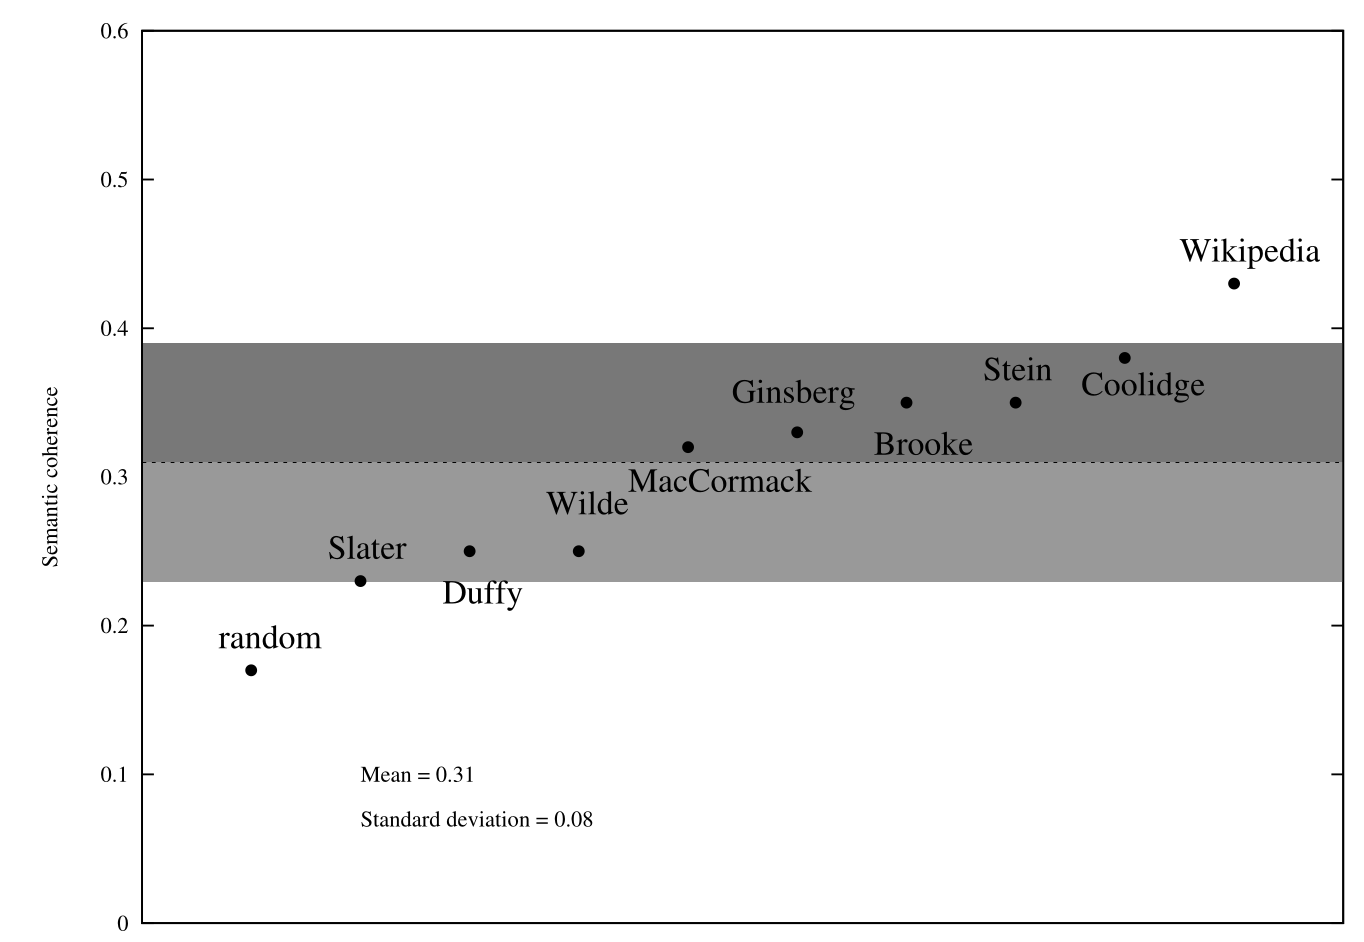
\includegraphics[scale=0.2]{../tex/img/coherence1.png}
  \caption{Coerența subiectelor din experimentul prezentat în \cite{herbelot}}
  \label{fig:coerenta1}
\end{figure}

}

\fr{
  \ft{Aplicație: Coerența semantică în poezia modernă}

  \begin{figure}[!htb]
  \centering
  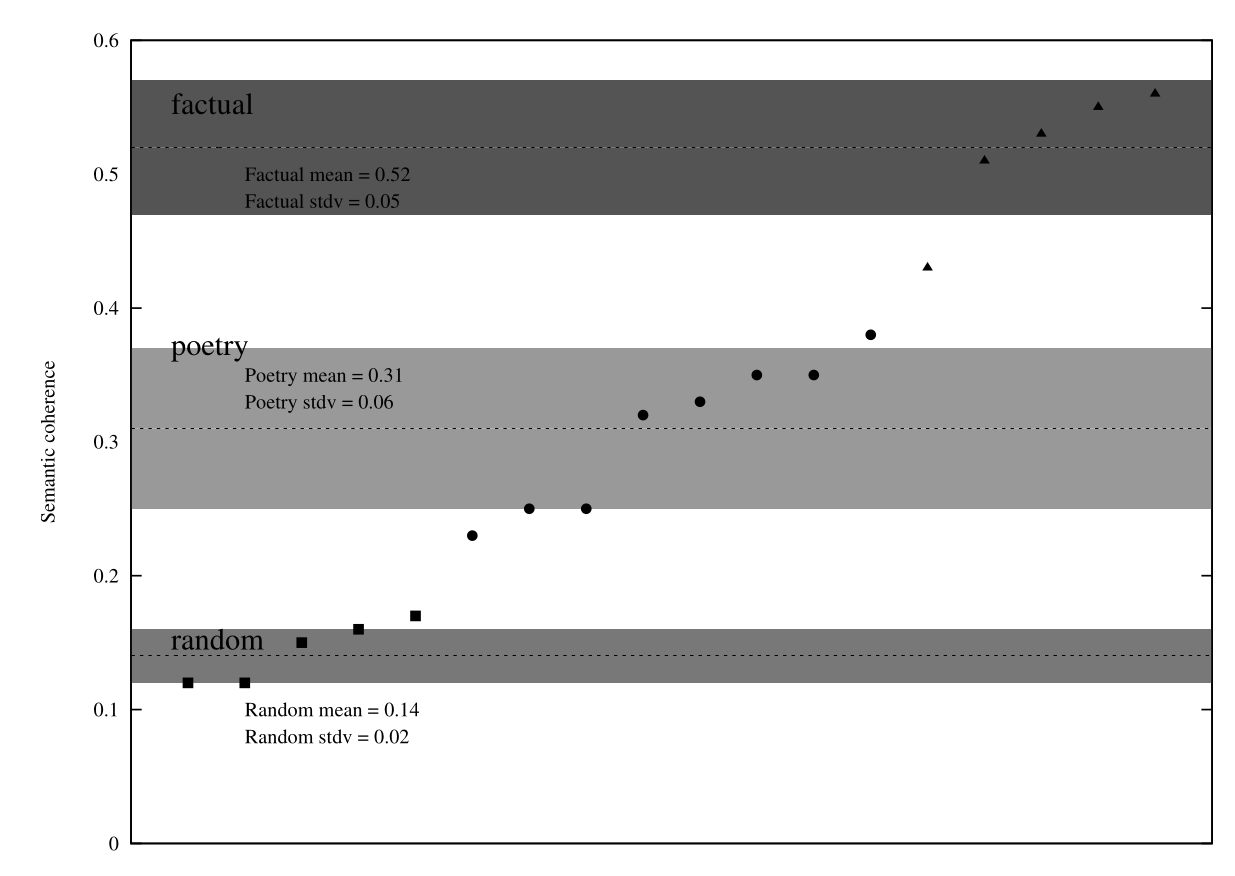
\includegraphics[scale=0.2]{../tex/img/coherence2.png}
  \caption{Coerența subiectelor din experimentul prezentat în \cite{herbelot},
  cu texte de control adăugate suplimentar}
  \label{fig:coerenta2}
\end{figure}
}

\fr{
  \ft{Aplicație: Coerența semantică în poezia modernă}

  \lin{1}{\textbf{Concluzii:}}{0}

  \begin{itemize}
    \ite{2}{Folosind SD, se poate vedea o relație între limbajul \qq{obișnuit}
      și cel \qq{neobișnuit} (al poeziei)};
    \ite{3}{Distincție clară între texte umane vs.\ generate aleatoriu}
    \ite{4}{Coerența poeziilor este \emph{între} texte aleatorii și texte științifice}
    \ite{5}{Coerența poeziilor nu {\small{(prea)}} depinde de dificultatea textului}
  \end{itemize}
}

\fr{
  \ft{Aplicație: Lord Byron vs.\ Thomas Moore 1813-1817}

  \lin{1}{Teza: Moore s-a inspirat de la Byron în poeziile din curentul
    \emph{orientalismului romantic}}{2}

  \lin{2}{Anti-teza: Genul literar are un vocabular și idei specifice,
    limitate $ \Rightarrow $ similaritatea este inevitabilă}{2}
}

\fr{
  \ft{Aplicație: Lord Byron vs.\ Thomas Moore 1813-1817}

  \lin{1}{Metoda: ESA (\emph{analiză semantică explicită})}{2}

  \lin{2}{Ideea: \qq{Se antrenează} semantic pe Wikipedia, apoi analizează
    textele date}{2}

  \lin{3}{Experimentul: cîte 4 poeme narative (mii de versuri), împărțite
    în grupuri de cîte $ \sim $ 200 versuri fiecare și se calculează
    scorul ESA}{2}

  \lin{4}{Model suplimentar: \qq{antrenare} pe 892 poeme narative}{2}
}

\fr{
  \ft{Aplicație: Lord Byron vs.\ Thomas Moore 1813-1817}

  \lin{1}{\textbf{Concluzii:}}{1}

  \begin{itemize}
    \ite{2}{Aproximativ 1000 perechi de versuri \qq{foarte legate}}
    \ite{3}{S-au analizat uman 15 perechi cu metoda Wikipedia și 15 perechi
      din modelul suplimentar}
    \ite{4}{Similaritățile sînt exact în zonele relevate de critici literari:
      personaje, sentimente și decoruri}
    \ite{5}{\emph{Dacă} a existat, inspirația dintre cei doi s-a manifestat unde
      s-a preconizat, DAR...}
    \ite{6}{Corpusul și textele nu sînt reprezentative; autorii recomandă
      rafinarea modelelor ESA și a corpusului înainte de concluzii clare}
    \ite{7}{\emph{Posibil} ca genul în sine să limiteze, să impună clișee}
  \end{itemize}
}
    
%%%%%%%%%%%%%%%%%%%%%%%%%%%%%%%%%%%%%%%%%%%%%%%%%%%%%%%%%%%%%%%%%%%%%%

% Bibliography
\begin{frame}[allowframebreaks]
    \ft{Bibliografie și lecturi suplimentare}
    \bibliography{../tex/semdis.bib}
    \bibliographystyle{apalike}
    \nocite{*}
\end{frame}

\end{document}

